\section{System enviroment configuration}
	\subsection{IntelliJ IDEA configuration}
A correct IntelliJ IDEA configuration needs to configure the path system\glo and after that to import an existing project.
	
	\begin{figure}[H]
		\centering
		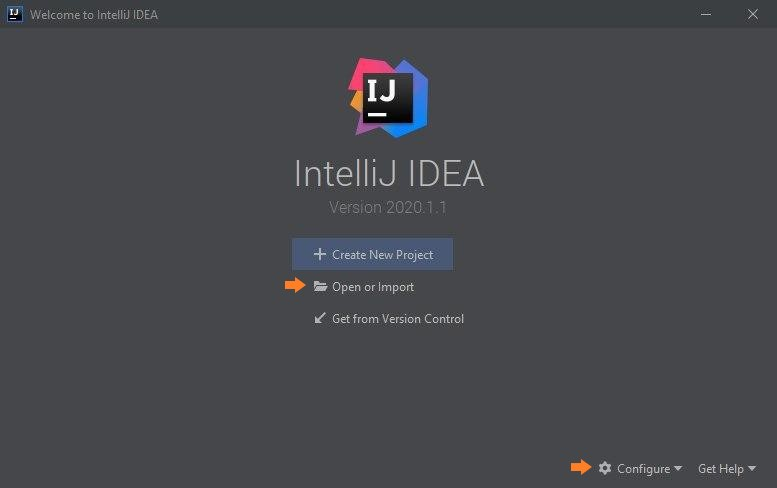
\includegraphics[scale=0.70]{../Developer_manual/img/intellijidea_main.jpg}
		\caption{IntelliJ IDEA first execution}
	\end{figure}	

	

	\subsubsection{Path system configuration}
Once you run IntelliJ IDEA move to "Configure" then "Settings"in the lower-right corner. Write "Node.js and NPM" in the search bar and check for the correct settings of fields "Node interpreter" and "Package manager", oherwise update them with the correct paths. 

\begin{figure}[H]
		\centering
		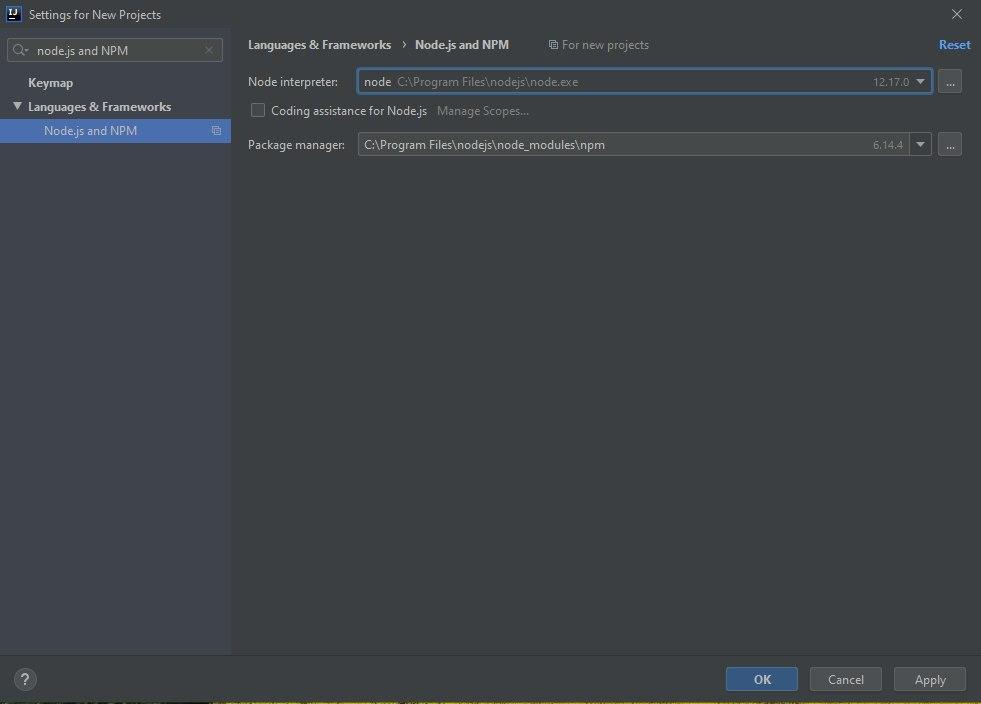
\includegraphics[scale=0.60]{../Developer_manual/img/nodejs_and_npm.jpg}
		\caption{Node.j and NPM settings}
	\end{figure}	

	\subsection{Project import}
From IntelliJ IDEA main window click on "Open or Import" and select the root directory of our project repository folder.

\begin{figure}[H]
		\centering
		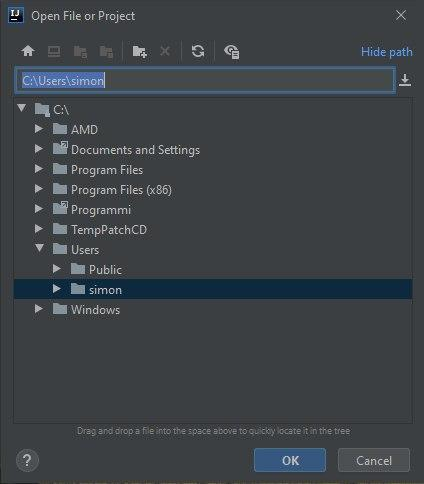
\includegraphics[scale=0.80]{../Developer_manual/img/open_project.jpg}
		\caption{Project path on opening}
	\end{figure}	


	\subsection{ESLint configuration}
		\subsubsection{Automatic configuration}
Since ESLint is listed as a dependency in our project IntelliJ IDEA automatically configures it. Move to "File" | "Settings" | "Languages and Frameworks" | "JavaScript" | "Code Quality Tools" | "ESLint" and check that Automatic ESLint configuration option is enabled. 


\begin{figure}[H]
		\centering
		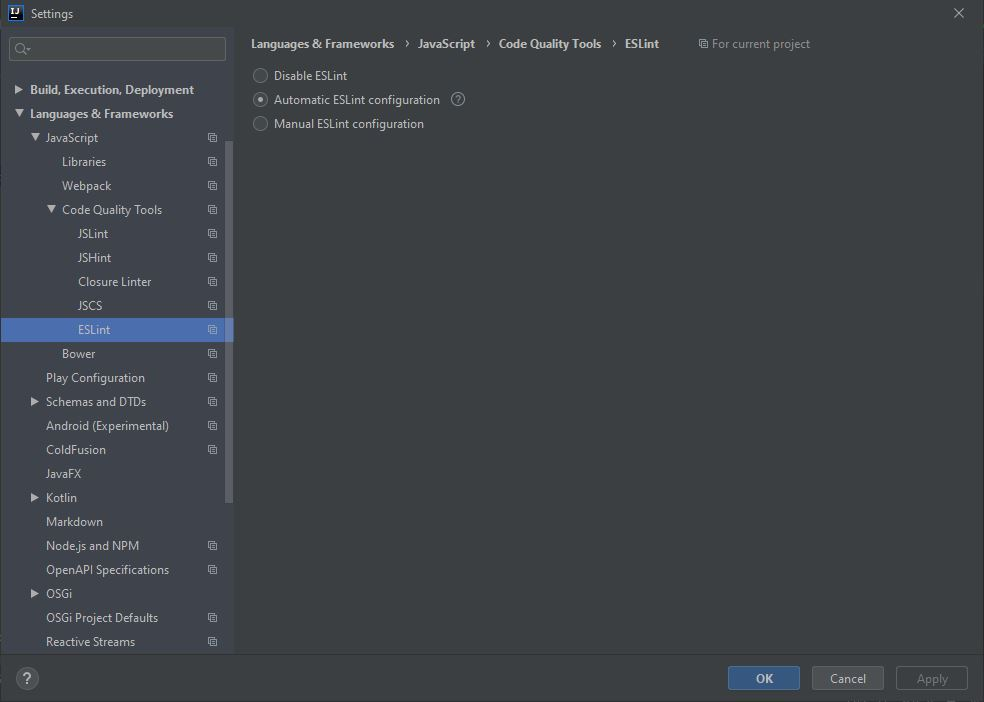
\includegraphics[scale=0.60]{../Developer_manual/img/automatic_eslint_configuration.JPG}
		\caption{Automatic ESLint configuration}
	\end{figure}	

		\subsubsection{Manual configuration}
You can also configure ESLint manually checking the Manual ESLint configuration option and complete fields as it follows:
		\begin{enumerate}
			\item in the "Node Interpreter" field, specify the path to Node.js;
			\item in the "ESLint Package" field, specify the location of the eslint or standard package;
			\item choose the configuration file to use checking "Automatic search" if you want to let IntelliJ IDEA do it for you or specify the file location in the path field;
			\item optionally specify additional command-line options to run ESLint in "Extra ESLint Options" field and specify the location of the files with additional code verification rules in the "Additional Rules Directory" field then confirm the whole configuration.
		\end{enumerate}
		

\begin{figure}[H]
		\centering
		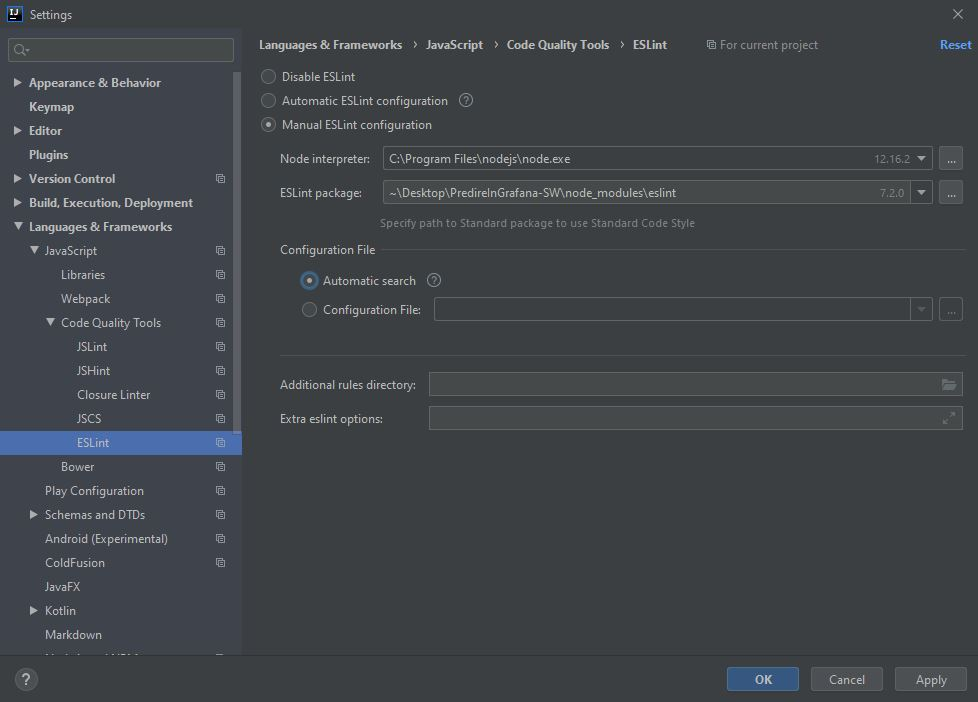
\includegraphics[scale=0.60]{../Developer_manual/img/manual_eslint_configuration.JPG}
		\caption{Manul ESLint configuration}
	\end{figure}	

	
	\subsection{Grafana plugin panel enviroment configuration}
	
	
		\subsubsection{package.json content}
In package.json file you can find all the app informations and requirements needed for its proper functioning. Attributes which represent important information are listed below:
		\begin{itemize}
			\item\textbf{scripts}: it contains all CLI command lines used from the developer: 
				\begin{itemize}
				\item\textbf{build}: this command creates a production-ready build of your plugin. It generates a folder named dist which contains our plugin production files ;
				\newline\texttt{npm run build}
				\item\textbf{test}: this command runs Jest against your codebase (used in automatic tests);
				\newline\texttt{npm run test}
				\item\textbf{dev} : this command creates a development build that's easy to play with and debug using common browser tooling;
				\newline\texttt{npm run dev}
				\item\textbf{watch}: this command run development task in a watch mode.
				\newline\texttt{npm run dev --watch}
			\end{itemize}
			\item\textbf{dependecies}: it contains the following packages needed for our app proper functioning:
			\begin{itemize}
				\item\textbf{@influxdata/influxdb-client}: the reference javascript client for InfluxDB. Both node and browser environments are supported;
    			\item\textbf{axios}: promise based HTTP client for the browser and node.js;
    			\item\textbf{react-files}: a file input (dropzone) management component for React we use when loading JSON files.
			\end{itemize}
			\item\textbf{devDependencies}: it contains the following packages needed for our app proper functioning during development:
			\begin{itemize}
				\item\textbf{@grafana/data}: a library containing most of the core functionality and data types used in Grafana.
				\item\textbf{@grafana-toolkit}: a CLI\glo that enables efficient development of Grafana plugins.
				\item\textbf{@grafana/ui}: a library containing the different design components of the Grafana ecosystem;
				\item\textbf{webpack}: used to compile JavaScript modules. Once installed, you can interface with webpack either from its CLI or API.
			\end{itemize}
		\end{itemize}
		
	\subsection{Training tool enviroment configuration}
	
	
		\subsubsection{package.json content}
In package.json file you can find all the app informations and requirements needed for its proper functioning. Attributes which represent important information are listed below:
		\begin{itemize}
			\item\textbf{scripts}: it contains all CLI command lines used from the developer: 
				\begin{itemize}
				\item\textbf{start}: the command runs the app in development mode. Open \texttt{http://localhost:3000} to view it in the browser. The page will automatically reload if you make changes to the code. You will see the build errors and lint warnings in the console;
				\newline\texttt{npm start}
				\item\textbf{build}: this command builds the app for production to the build folder. It correctly bundles React in production mode and optimizes the build for the best performance. The build is minified and the filenames include the hashes. In the end our app is ready to be deployed;
				\newline\texttt{npm run build}
				\item\textbf{test}: this command runs the test watcher in an interactive mode. By default, runs tests related to files changed since the last commit.
				\newline\texttt{npm test}
				\item\textbf{eject}: this command will copy all the configuration files and the transitive dependencies into our project as dependencies in package.json ;
				\newline\texttt{npm run eject}
			\end{itemize}
			\item\textbf{dependecies}: it contains the following packages needed for our app proper functioning:
			\begin{itemize}
				\item\textbf{@testing-library/react}: simple and complete React DOM testing utilities that encourage good testing practices. ;
    			\item\textbf{@testing-library/user-event}: simulate user events for react-testing-library;
    			\item\textbf{bootstrap}: sleek, intuitive, and powerful front-end framework for faster and easier web development;
    			\item\textbf{chart.js}: simple yet flexible JavaScript charting for designers and developers;
    			\item\textbf{is-promise}: test whether an object looks like a promises-a+ promise;
    			\item\textbf{libsvm-js}: c++ library that allows to do Support Vector Machine classification and regression;
    			\item\textbf{ml-svm}: Support Vector Machine in Javascript;
    			\item\textbf{react}: JavaScript library for creating user interfaces. The react package contains only the functionality necessary to define React components;
    			\item\textbf{react-bootstrap}: bootsrap components built with React;
				\item\textbf{react-chartjs-2}: React wrapper for Chart.js 2;     			
    			\item\textbf{react-csv-reader}: React component that handles csv file input. It handles file input and returns its content as a matrix;
    			\item\textbf{react-dom}: package that serves as the entry point to the DOM and server renderers for React. It is intended to be paired with the generic React package, which is shipped as react to npm;
    			\item\textbf{react-scripts}: this package includes scripts and configuration used by Create React App;
    			\item\textbf{svm}: is a lightweight implementation of the SMO algorithm to train a binary Support Vector Machine. As this uses the dual formulation, it also supports arbitrary kernels. 
			\end{itemize}
			\item\textbf{devDependencies}: it contains the following packages needed for our app proper functioning during development:
			\begin{itemize}
				\item\textbf{@testing-library/jest-dom}: custom jest matchers to test the state of the DOM;
				\item\textbf{csv-parser}: streaming CSV parser that aims for maximum speed as well as compatibility with the csv-spectrum CSV acid test suite. Csv-parser can convert CSV into JSON;
				\item\textbf{eslint-plugin-react-hooks}: this ESLint plugin enforces the Rules of Hooks. It is a part of the Hooks API for React.

			\end{itemize}
		\end{itemize}
		